\chapter{Photonen und die Zukunft der Physik}
\setcounter{section}{7}
\setcounter{subsection}{0}
\setcounter{subsubsection}{1}
\setcounter{secnumdepth}{3}
% Boxen-Stile definieren
\tcbset{physikbox/.style={colback=blue!5!white, colframe=blue!75!black, fonttitle=\bfseries}}
\tcbset{mathebox/.style={colback=green!5!white, colframe=green!50!black, fonttitle=\bfseries}}
\tcbset{didaktikbox/.style={colback=yellow!5!white, colframe=yellow!50!black, fonttitle=\bfseries}}
\tcbset{hypobox/.style={colback=orange!5!white, colframe=orange!75!black, fonttitle=\bfseries}}
\tcbset{hinweisbox/.style={colback=gray!10!white, colframe=black!40!black, fonttitle=\bfseries}}

\subsection{Einleitung}
\index{Photon}
\index{Photonik}
\index{Kommunikation}
\index{Messtechnik}
\index{Datenverarbeitung}
\index{Photonischer Computer}
\index{Quantenkommunikationsnetz}
\index{Graviton}
\index{Dunkle Energie}
\index{Standardmodell}

Photonen prägen nicht nur unsere heutige Technologie, sondern öffnen auch Türen zu völlig neuen Forschungsfeldern. 
Während sie in der Kommunikation, Messtechnik und Datenverarbeitung bereits unverzichtbar sind, stehen wir zugleich am Beginn einer Ära, in der Photonen zentrale Rollen in photonischen Computern, Quantenkommunikationsnetzen und präzisesten Experimenten der Grundlagenforschung übernehmen.  
Dieses Kapitel spannt den Bogen von aktuellen Entwicklungen in der Photonik über zukunftsweisende Anwendungen bis hin zu den großen offenen Fragen der Physik – von der Suche nach dem hypothetischen Graviton über das Rätsel der Dunklen Energie bis zu möglichen Erweiterungen des Standardmodells. 
Die vorgestellten Themen zeigen, wie das kleinste Quantenobjekt des Lichts zum Schlüssel für die Technologien und Entdeckungen von morgen werden könnte.
\begin{figure}[H]
	\centering
	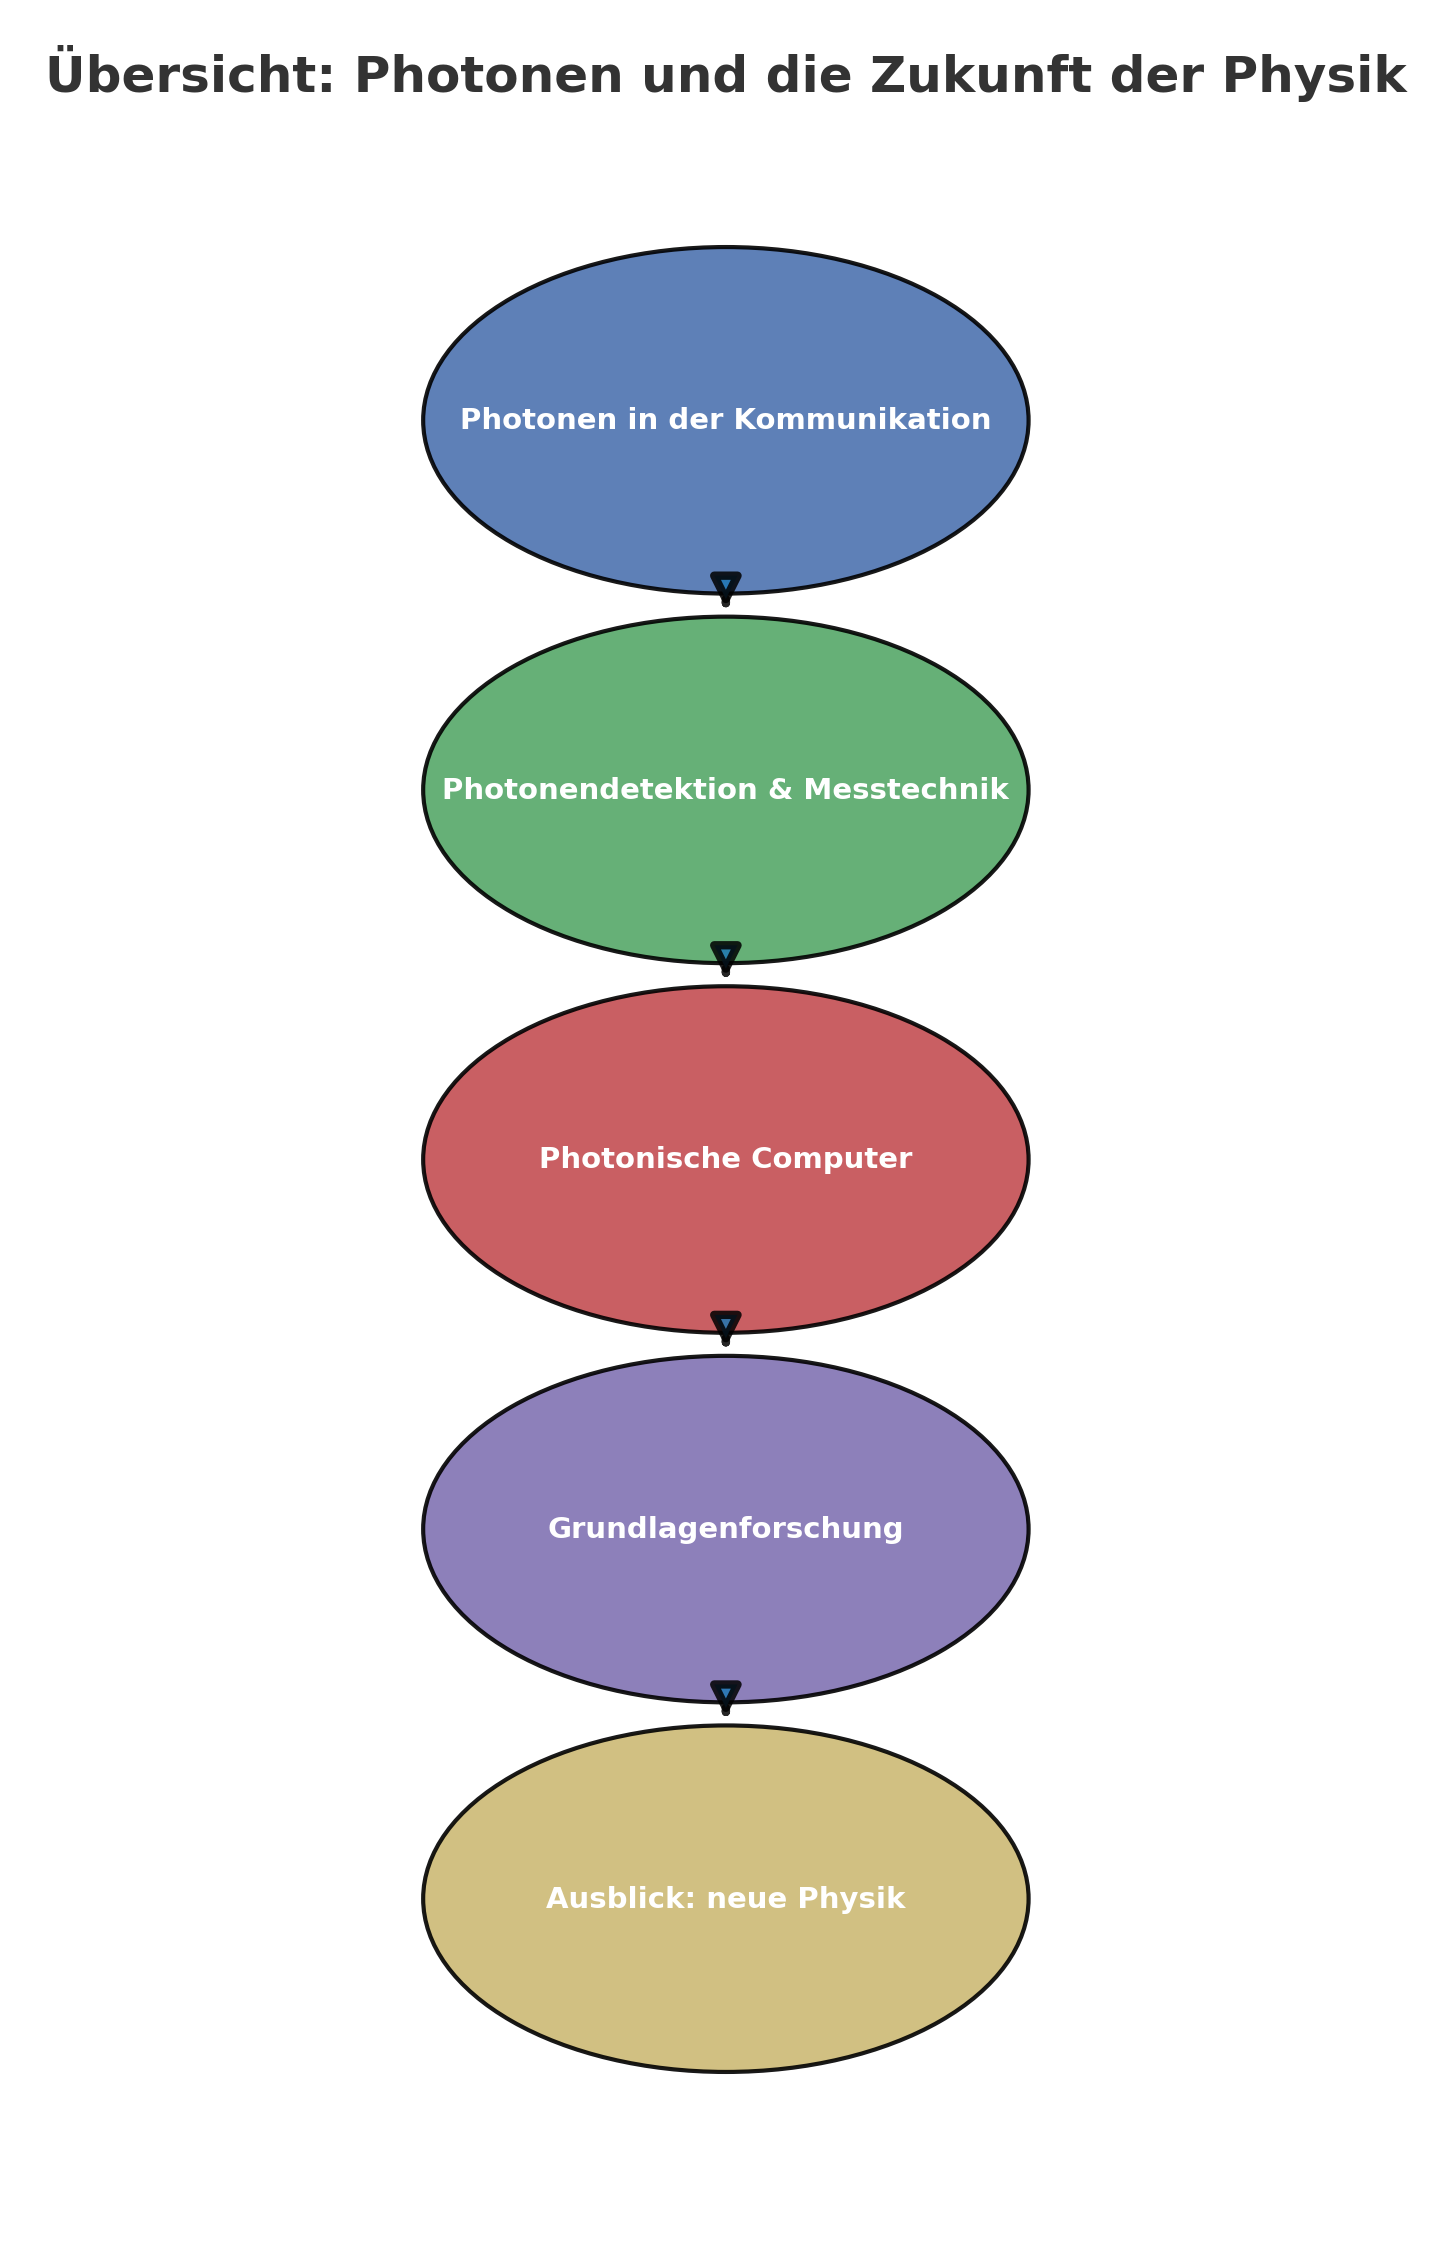
\includegraphics[width=0.75\textwidth]{bilder/kapitel_VII_uebersicht.png}
	\caption[Übersicht Kapitel~VII]{Übersicht: Photonen und die Zukunft der Physik. 
		Die Grafik zeigt die Hauptthemen dieses Kapitels in einer vertikalen Anordnung, 
		von photonischer Logik bis zu offenen Fragen neuer Physik.}
	\label{fig:kapitel_VII_uebersicht}
\end{figure}

\subsection{Einzelphotonen und Quanteninformation}
\index{Einzelphoton}
\index{Quanteninformation}
\index{Qubit}
\index{Superposition}
\index{Polarisation}
\index{Zeit-Bin}
\index{Frequenzkodierung}

Die Fähigkeit, einzelne Photonen gezielt zu erzeugen, zu steuern und zu detektieren, hat in den letzten Jahren eine Schlüsselrolle in der Quanteninformationstechnologie eingenommen. Einzelphotonen dienen als ideale Träger quantenmechanischer Information: Sie sind robust gegenüber Störungen, bewegen sich mit Lichtgeschwindigkeit\index{Lichtgeschwindigkeit} und lassen sich in wohldefinierten Quantenzuständen\index{Quantenzustand} präparieren.

In der klassischen Informationstechnik werden Bits in Form von elektrischen Spannungen oder magnetischen Zuständen gespeichert und verarbeitet. In der Quanteninformation dagegen basiert die kleinste Informationseinheit — das \emph{Qubit} — auf der kohärenten Superposition\index{Superposition} von Zuständen. Bei Photonen werden diese Zustände oft durch Polarisationsrichtungen, Zeit-Bins oder Pfadinformationen realisiert.
\vspace{1em}
\begin{tcolorbox}[physikbox, title=Was macht ein Photon zum Informationsträger? \label{box:photon_information}]
	\small
	Photonen können verschiedene physikalische Freiheitsgrade tragen, die als Qubits nutzbar sind:
	\begin{itemize}
		\item \textbf{Polarisation:} Horizontal ($\ket{H}$) und vertikal ($\ket{V}$) als Basiszustände.
		\item \textbf{Zeit-Bins:} Frühe und späte Ankunftszeiten als logische Zustände.
		\item \textbf{Ort/Pfad:} Zwei verschiedene optische Wege in einem Interferometer\index{Interferometer}.
		\item \textbf{Frequenz:} Unterschiedliche spektrale Modi für kodierte Information.
	\end{itemize}
	Diese Freiheitsgrade lassen sich präzise kontrollieren und über große Distanzen übertragen, ohne dass die Quanteninformation zerstört wird.
\end{tcolorbox}

\subsubsection{Erzeugung von Einzelphotonen}
\index{Einzelphotonenquelle}
\index{Spontane parametrische Fluoreszenz}
\index{Einzelatom}
\index{Ion}
\index{Quantenpunkt}
\index{nichtlinearer Kristall}
\index{Halbleitermaterial}

Einzelphotonenquellen sind zentrale Bausteine der Quantenoptik\index{Quantenoptik}. Gängige Methoden sind:
\begin{itemize}
	\item \emph{Spontane parametrische Fluoreszenz} (SPDC) in nichtlinearen Kristallen.
	\item \emph{Einzelatome} oder Ionen in optischen Fallen\index{optische Falle}.
	\item \emph{Quantenpunkte} in Halbleitermaterialien.
\end{itemize}
Ziel ist es, Photonen mit hoher Reinheit (geringe Mehrphotonenwahrscheinlichkeit) und hoher Indistinguishability (Unterscheidbarkeit) zu erzeugen.
\vspace{1em}
\begin{tcolorbox}[hinweisbox, title=Was bedeutet „Indistinguishability“? \label{box:indistinguishability}]
	\small
	In der Quantenoptik beschreibt \emph{Indistinguishability}, dass zwei Photonen in allen physikalischen Eigenschaften ununterscheidbar sind:
	\begin{itemize}
		\item gleiche Frequenz (Energie)
		\item gleiche Polarisation
		\item identischer räumlicher Modus (gleicher Strahlweg)
		\item identische Ankunftszeit innerhalb der Kohärenzzeit
	\end{itemize}
	Nur wenn Photonen vollkommen indistinguishabel sind, können sie quantenmechanische Interferenzeffekte wie das \emph{Hong–Ou–Mandel-Dip}-Phänomen zeigen.
\end{tcolorbox}
\vspace{1em}
\begin{tcolorbox}[physikbox, title=Das Hong–Ou–Mandel-Dip-Phänomen \label{box:hong_ou_mandel}]
	\small
	Das \emph{Hong–Ou–Mandel-Dip}-Experiment ist ein zentrales Verfahren, um die \emph{Indistinguishability} zweier Photonen zu überprüfen. Treffen zwei ununterscheidbare Photonen gleichzeitig auf einen 50:50-Strahlteiler, verlassen sie diesen stets gemeinsam durch denselben Ausgang — ein reiner Quanteninterferenzeffekt.  
	Die Tiefe des gemessenen „Dips“ in der Koinzidenzrate ist ein direktes Maß für die Ununterscheidbarkeit der Photonen.  
	Eine ausführliche Beschreibung und Abbildung findet sich in \textbf{Kapitel IV.5}.
\end{tcolorbox}

\subsubsection{Dekohärenz und Fehlerquellen}
\index{Dekohärenz}
\index{Quantenfehlerkorrektur}
\index{Quantenrepeater}
\index{Faserdämpfung}
\index{Streuung}
\index{Phasenrauschen}
\index{Vibration}

Quanteninformation ist empfindlich gegenüber Störungen. Bei Photonen sind die Hauptursachen für Dekohärenz:
\begin{itemize}
	\item Wechselwirkung mit dem Übertragungsmedium (z.\,B. Faserdämpfung, Streuung).
	\item Phasenrauschen durch Temperaturschwankungen und Vibrationen.
\end{itemize}
Fehlerkorrektur und Quantenrepeater sind notwendig, um Quanteninformation über weite Strecken zu erhalten.
\newpage
\noindent
\subsubsection{Anwendungen}
\index{Quantenkryptographie}
\index{Satellitenkommunikation}
\index{Hybrid-Quantensystem}

Einzelphotonen bilden die Grundlage für:
\begin{itemize}
	\item Quantenkryptographie.
	\item Quantenkommunikation über Satelliten.
	\item Hybride Systeme, in denen Photonen als Schnittstelle zwischen Materie-Qubits dienen.
\end{itemize}
Diese Anwendungen markieren den Beginn einer neuen Ära der Informationsverarbeitung, in der Photonen nicht nur Träger, sondern auch Vermittler zwischen unterschiedlichen Quantensystemen sind.

\subsection{Quantenkryptographie und Quantenkommunikation} \label{sec:quantum_crypto}
\index{RSA}
\index{Quantencomputer}
\index{Quantenkryptographie}
\index{Quantenkommunikation}
\index{Heisenbergsche Unschärferelation}
\index{No-Cloning-Theorem}
\index{BB84-Protokoll}
\index{Bennett, Charles}
\index{Brassard, Gilles}
\index{Quanten-Schlüsselverteilung}
\index{Satellitenbasierte Quantenkommunikation}
\index{Micius}

Die Sicherheit klassischer Kommunikationssysteme basiert auf mathematischen Verfahren, deren Sicherheit auf der praktischen Unmöglichkeit bestimmter Berechnungen beruht — etwa der Faktorisierung großer Zahlen bei RSA. Diese Sicherheit kann durch zukünftige Quantencomputer gefährdet werden.  
Die Quantenkryptographie hingegen nutzt fundamentale physikalische Gesetze, um die Sicherheit zu gewährleisten — unabhängig von der Rechenleistung eines Angreifers.
\vspace{1em}
\begin{tcolorbox}[physikbox, title=Kernprinzip der Quantenkryptographie \label{box:qcrypto_prinzip}]
	\small
	Die Quantenkryptographie beruht auf zwei zentralen Eigenschaften der Quantenmechanik:
	\begin{enumerate}
		\item \textbf{Messstörung:} Jeder Messversuch an einem Quantenzustand verändert diesen (Heisenbergsche Unschärferelation).
		\item \textbf{Nicht-Klonbarkeit:} Unbekannte Quantenzustände können nicht verlustfrei kopiert werden (No-Cloning-Theorem).
	\end{enumerate}
	Daraus folgt: Abhören hinterlässt unausweichlich Spuren, die von den legitimen Kommunikationspartnern erkannt werden können.
\end{tcolorbox}
\newpage
\noindent
\subsubsection{Quanten-Schlüsselverteilung (QKD)}

Das bekannteste Protokoll ist \textbf{BB84} (Bennett \& Brassard, 1984). Dabei werden einzelne Photonen in zufälligen Polarisationszuständen übertragen.  
Der Ablauf in Kurzform:
\begin{itemize}
	\item Sender (\emph{Alice}) wählt zufällig eine von zwei möglichen Basen (z.\,B. horizontal/vertikal oder diagonal).
	\item Empfänger (\emph{Bob}) misst in zufällig gewählten Basen.
	\item Nach der Übertragung vergleichen beide öffentlich ihre Basiswahl und verwerfen Messungen, bei denen die Basen nicht übereinstimmen.
	\item Aus den verbleibenden Daten wird ein gemeinsamer Schlüssel extrahiert.
\end{itemize}
Ein Abhörversuch (\emph{Eve}) führt zu zusätzlichen Fehlern, die statistisch nachweisbar sind.

\subsubsection{Quantenkommunikation über große Distanzen}

Die Reichweite direkter Quantenkommunikation ist durch Verluste in Glasfasern\index{Glasfaser} und durch atmosphärische Störungen\index{Atmosphäre} begrenzt. Mögliche Lösungen sind:
\begin{itemize}
	\item \textbf{Quantenrepeater:} Knotenpunkte, die verschränkte Photonenpaare\index{verschränkte Photonen} erzeugen und über große Entfernungen verteilen.
	\item \textbf{Satellitenbasierte Quantenkommunikation:} Umgehung der Faserverluste durch freie Übertragung im Weltraum (z.\,B. der chinesische Quantenkommunikationssatellit \emph{Micius}).
\end{itemize}

\subsubsection{Anwendungen und Ausblick}

Quantenkryptographie wird derzeit für hochsichere Regierungs- und Finanzkommunikation getestet. In Kombination mit klassischen Netzwerken entstehen hybride Systeme, die langfristig sichere Kommunikation auch im Zeitalter der Quantencomputer ermöglichen sollen.

Bemerkenswert ist dabei die doppelte Rolle der Quantenphysik:  
Einerseits bedrohen Quantencomputer durch ihre Rechenleistung die Sicherheit heutiger Verschlüsselungsverfahren.  
Andererseits liefert dieselbe Physik mit der Quantenkryptographie einen völlig neuen Ansatz, der prinzipiell abhörsichere Kommunikation erlaubt.  
Dieses Wechselspiel zwischen Herausforderung und Lösung macht die Quantenkommunikation zu einem der spannendsten Forschungsfelder der modernen Physik.

\subsection{Photonik als Zukunftstechnologie}
\index{Laser}
\index{LED}
\index{Glasfaser}
\index{Photonischer Chip}
\index{Photonendetektor}
\index{Modulator}
\index{Filter}
\index{nichtlinearer Kristall}

Photonen sind nicht nur fundamentale Informationsträger in der Quantenphysik, sondern bilden auch die Grundlage zahlreicher moderner Technologien.  
Die \emph{Photonik} umfasst alle Technologien, die auf der Erzeugung, Kontrolle und Detektion von Licht basieren – vom Laser in der Medizin bis zur Glasfaser im weltweiten Kommunikationsnetz.
\vspace{1em}
\begin{tcolorbox}[hinweisbox, title=Was bedeutet „Photonik“? \label{box:photonics_definition}]
	\small
	Der Begriff \emph{Photonik} beschreibt den ingenieurwissenschaftlichen und technologischen Umgang mit Photonen – analog zur Elektronik, die sich mit Elektronen beschäftigt.  
	Photonik umfasst:
	\begin{itemize}
		\item Lichtquellen (Laser, LEDs, Quantenlichtquellen)
		\item Lichtführung (Glasfaser, photonische Chips)
		\item Lichtdetektion (Kameras, Photonendetektoren)
		\item Lichtmanipulation (Modulatoren, Filter, nichtlineare Kristalle)
	\end{itemize}
\end{tcolorbox}

%index
\subsubsection{Photonik in der Kommunikation}
\index{Telekommunikation}
\index{Photonischer Schalter}
\index{Router}
\index{Mikrochip}

In der Telekommunikation ersetzt Photonik zunehmend die Elektronik, um die steigenden Datenmengen zu bewältigen. Glasfasernetze übertragen Informationen mit Lichtgeschwindigkeit und minimalem Energieverlust.  
Photonische Schalter und Router auf Mikrochips versprechen ultraschnelle Signalverarbeitung direkt mit Photonen.

\subsubsection{Photonik in der Medizin}
\index{Laserchirurgie}
\index{optische Kohärenztomographie}
\index{Fluoreszenzdiagnostik}
\index{Biosensor}

Photonische Verfahren wie Laserchirurgie, optische Bildgebung (OCT) und fluoreszenzbasierte Diagnostik haben die Medizin revolutioniert.  
Zukünftige Entwicklungen umfassen minimalinvasive Operationen mit ultrakurzen Laserpulsen und photonische Biosensoren für Echtzeitdiagnosen.

\subsubsection{Photonik in der Sensorik und Messtechnik}
\index{Photonischer Sensor}
\index{LIDAR}
\index{Gravitationswellendetektor}

Photonische Sensoren ermöglichen hochpräzise Messungen in Industrie, Geowissenschaften und Raumfahrt.  
Beispiele sind LIDAR-Systeme für autonomes Fahren und interferometrische Gravitationswellendetektoren.

\vspace{1em}
\begin{tcolorbox}[physikbox, title=Photonische Schaltungen vs. Elektronische Schaltungen \label{box:photon_vs_electron}]
	\small
	Photonische Schaltungen bieten gegenüber elektronischen Ansätzen mehrere entscheidende Vorteile:
	\begin{itemize}
		\item \textbf{Höhere Geschwindigkeit:} Licht bewegt sich im Medium deutlich schneller als Elektronen in Leitern.
		\item \textbf{Geringere Verluste:} Keine ohmsche Erwärmung durch elektrischen Widerstand.
		\item \textbf{Höhere Bandbreite:} Ein Photonensignal kann viele Wellenlängen (Multiplexing) gleichzeitig tragen.
		\item \textbf{Geringe Übersprechung:} Kaum elektromagnetische Störeinflüsse zwischen benachbarten Leitungen.
	\end{itemize}
	Diese Eigenschaften machen photonische Schaltungen zu einem Schlüsselfaktor für zukünftige Hochgeschwindigkeits- und Hochbandbreitentechnologien.
\end{tcolorbox}

\subsubsection{Ausblick}

Photonik gilt als Schlüsseltechnologie des 21. Jahrhunderts. Ihre Kombination mit der Quantenphysik – etwa in Quantenkommunikation, Quantencomputern oder Quantenmetrologie – verspricht völlig neue Anwendungen.  
Die Entwicklung hin zu integrierten photonischen Schaltkreisen könnte in der Informationsverarbeitung einen ähnlichen Umbruch auslösen wie die Mikroelektronik im 20. Jahrhundert.

\subsection{Optische Logik und photonische Computer}
\index{Optische Logik}
\index{Mach--Zehnder-Interferometer}
\index{Mikroresonator}
\index{Optischer Modulator}

Die Miniaturisierung elektronischer Schaltkreise stößt zunehmend an physikalische Grenzen: Transistoren werden so klein, dass Quanten- und Wärmeeffekte ihre Funktion beeinträchtigen. Gleichzeitig steigt der Energiebedarf moderner Rechenzentren rasant. Eine vielversprechende Alternative ist die Nutzung von Photonen anstelle von Elektronen zur Informationsverarbeitung.
\vspace{1em}
\begin{tcolorbox}[physikbox, title=Warum Photonen für Logikschaltungen interessant sind, label=box:optlogik_vorteile]
	\small
	\begin{itemize}
		\item \textbf{Hohe Geschwindigkeit:} Licht bewegt sich nahezu mit Lichtgeschwindigkeit – optische Signale können extrem schnell verarbeitet werden.
		\item \textbf{Keine ohmschen Verluste:} Im Gegensatz zu elektrischen Strömen erwärmen sich optische Leitungen kaum.
		\item \textbf{Parallele Verarbeitung:} Durch Multiplexing können mehrere Wellenlängen gleichzeitig genutzt werden.
		\item \textbf{Direkte Kopplung an Glasfaser-Kommunikation:} Keine Umwandlung zwischen Elektronen- und Photonen-Signalen nötig.
	\end{itemize}
\end{tcolorbox}

\subsubsection{Grundprinzip optischer Logikgatter}
\index{Optisches Logikgatter}
\index{Photonischer Kristall}

Optische Logikschaltungen arbeiten mit Bauelementen, die Lichtstrahlen abhängig von Eingangsbedingungen umleiten, abschwächen oder verstärken. Beispiele sind nichtlineare Kristalle, optische Modulatoren oder photonische Kristallstrukturen.  
Logikgatter wie \textsc{AND}, \textsc{OR} und \textsc{NOT} lassen sich dabei durch Interferenz, Absorption oder Polarisationsänderung realisieren.
\vspace{1em}
\begin{tcolorbox}[didaktikbox, title=Von Elektronik zu Photonik]
	\label{box:optlogik_didaktik}
	\small
	In der Elektronik basieren Logikgatter auf Transistoren, die den Stromfluss blockieren oder freigeben. In der Photonik übernehmen Bauelemente wie Mach–Zehnder-Interferometer oder Mikroresonatoren diese Aufgabe – nur eben für Licht.
\end{tcolorbox}

\subsubsection{Photonische Computer}
\index{Photonischer Computer}
\index{Künstliche Intelligenz}
\index{Signalverarbeitung}
\index{Quanteninformationsverarbeitung}

Ein photonischer Computer nutzt optische Schaltungen für zentrale Rechenoperationen. Besonders geeignet ist diese Technik für:
\begin{itemize}
	\item \textbf{Künstliche Intelligenz:} Matrixmultiplikationen können extrem schnell und energieeffizient in optischen Netzwerken durchgeführt werden.
	\item \textbf{Signalverarbeitung:} Breitbandige Verarbeitung ohne elektrische Engpässe.
	\item \textbf{Quanteninformationsverarbeitung:} Kombination aus photonischer Logik und Quantenbits (Qubits).
\end{itemize}
\vspace{1em}
\begin{tcolorbox}[hypobox, title={Was wäre, wenn optische Computer Elektronik ablösen?}]
	\label{box:optlogik_zukunft}
	\small
	Falls photonische Computer die Elektronik vollständig ersetzen könnten, ließe sich der Energieverbrauch großer Rechenzentren drastisch senken. Gleichzeitig könnten Taktraten im Terahertz-Bereich erreicht werden – weit jenseits heutiger Prozessoren.
\end{tcolorbox}
Optische Logikgatter lassen sich auch mit einem Mach–Zehnder-Interferometer (MZI) realisieren. 
Dabei teilt ein Strahlteiler den Laserstrahl in zwei Pfade, in denen jeweils ein Phasenmodulator sitzt. 
Nur wenn beide Modulatoren eine bestimmte Phasenverschiebung setzen, interferieren die beiden Strahlen am zweiten Strahlteiler so, dass Licht am gewünschten Ausgang erscheint. 
Wählt man die Phasen so, dass dies nur bei zwei aktiven Eingaben geschieht, arbeitet das MZI wie ein klassisches \textsc{AND}-Gatter – allerdings auf rein optischem Weg. 
%Eine kompakte Wahrheitstabelle und die genaue Funktionsweise sind in \ref{sec:mzi_and_detail} beschrieben.
\vspace{1em}
\begin{tcolorbox}[didaktikbox, title=Photonisches AND-Gatter im Mach--Zehnder-Interferometer, label={box:mzi_and}]
	\small
	Ein Mach--Zehnder-Interferometer kann so beschaltet werden, dass es wie ein \textsc{AND}-Gatter arbeitet. 
	Die Eingänge \(A\) und \(B\) steuern Phasenmodulatoren in den beiden Armen des Interferometers. 
	Nur wenn beide eine Phasenverschiebung von \(\pi\) setzen, addieren sich die Phasen zu \(2\pi\) und es kommt zu konstruktiver Interferenz am „1“-Ausgang.
	
	\begin{center}
		\begin{tabular}{c c c c c c}
			\toprule
			\(A\) & \(B\) & Phase A & Phase B & Ausgang „1“ & Ausgang „0“ \\
			\midrule
			0 & 0 & \(0\) & \(0\) & 1 & 0 \\
			0 & 1 & \(0\) & \(\pi\) & 0 & 1 \\
			1 & 0 & \(\pi\) & \(0\) & 0 & 1 \\
			1 & 1 & \(\pi\) & \(\pi\) & 1 & 0 \\
			\bottomrule
		\end{tabular}
	\end{center}
	
	Nur bei \(A=1\) und \(B=1\) ist die Gesamtphase \(2\pi\), sodass der obere Ausgang hell wird. 
	In allen anderen Fällen wird das Licht in den „0“-Ausgang gelenkt.
\end{tcolorbox}
\begin{figure}[H]
	\centering
	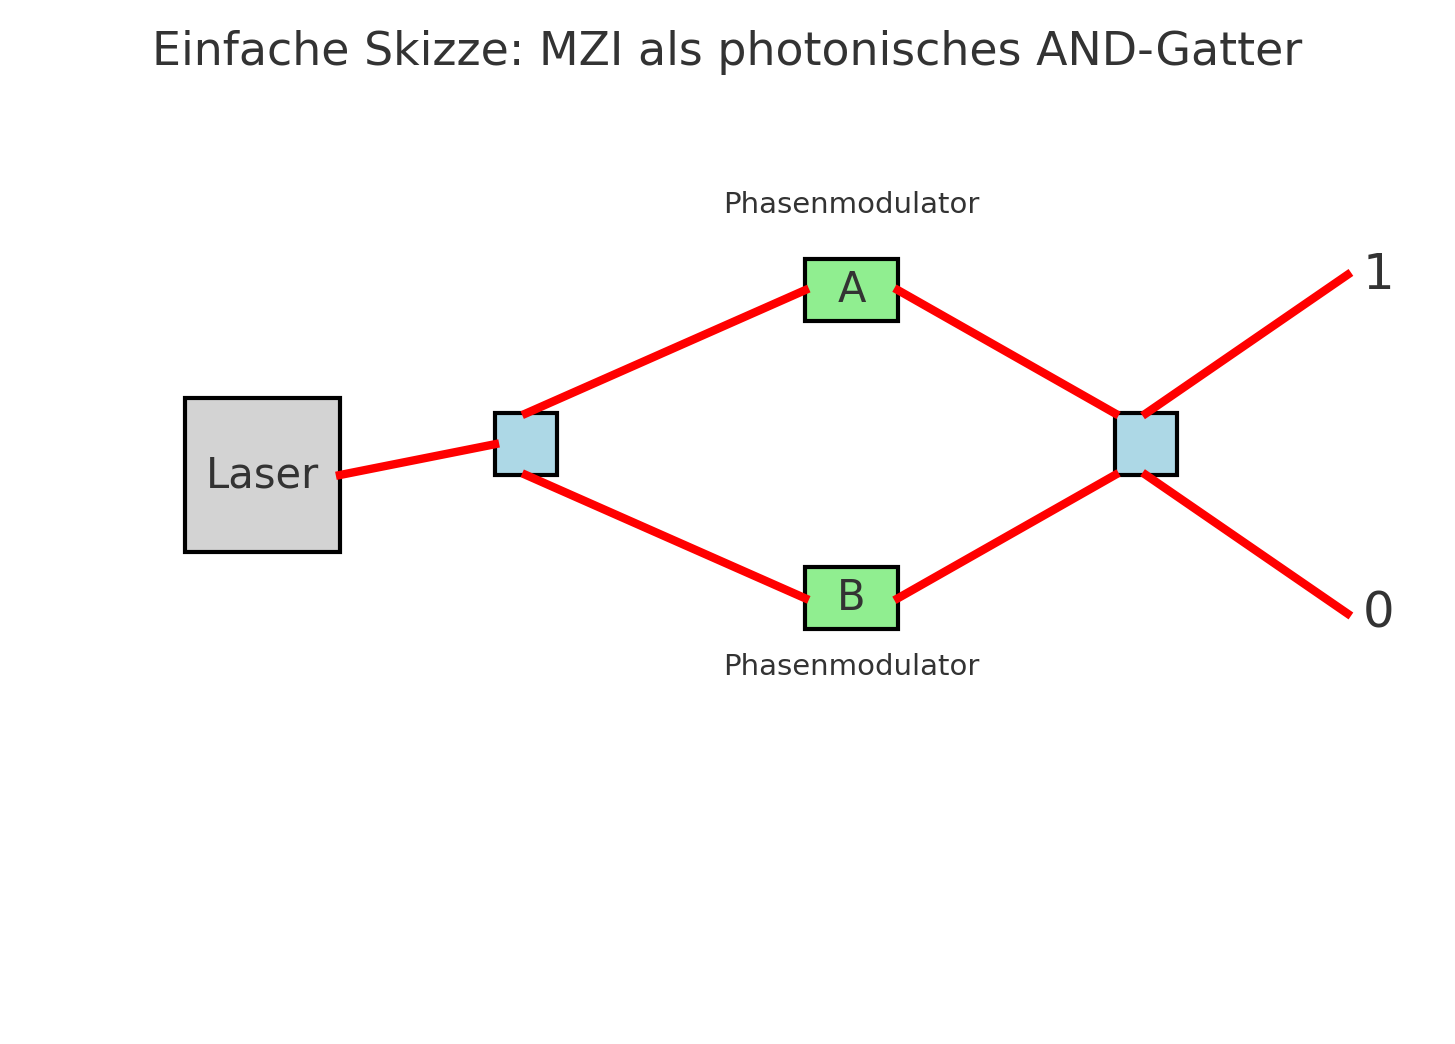
\includegraphics[width=0.75\textwidth]{bilder/mzi_and_simple.png} % <-- Pfad anpassen
	\caption{Einfache schematische Darstellung eines Mach--Zehnder-Interferometers mit zwei Phasenmodulatoren (\(A\) und \(B\)), das als photonisches \textsc{AND}-Gatter arbeitet. Nur wenn beide Modulatoren eine Phasenverschiebung von \(\pi\) setzen, addieren sich die Phasen zu \(2\pi\) und es erscheint Licht am „1“-Ausgang.}
	\label{fig:mzi_and_simple}
\end{figure}

\subsubsection{Herausforderungen}
\index{Chip-Integration}
\index{Miniaturisierung}
\index{Elektronik-Integration}

Trotz der Vorteile gibt es noch offene Probleme:
\begin{itemize}
	\item Effiziente Erzeugung und Kontrolle einzelner Photonen auf Chip-Ebene.
	\item Miniaturisierung optischer Bauteile auf Nanometermaßstab.
	\item Integration mit bestehender Elektronik.
\end{itemize}

\subsubsection{Zusammenfassung}

Optische Logik und photonische Computer bieten eine faszinierende Möglichkeit, die Rechenleistung zu steigern und den Energiebedarf zu senken. Ob sie die klassische Elektronik komplett ablösen oder nur in Spezialanwendungen dominieren werden, hängt von der Lösung der technischen Herausforderungen ab.
\newpage
\noindent
\subsection{Photonen in der Grundlagenforschung}
\index{Boson}
\index{Kosmologie}
\index{Kosmischer Mikrowellenhintergrund}
\index{Bell-Test}
\index{Quantentomographie}
\index{Gravitationslinse}
\index{Lorentz-Invarianz}
\index{CPT-Symmetrie}

Photonen spielen nicht nur in der Technik, sondern auch in der modernen Grundlagenforschung eine zentrale Rolle. 
Ihre Eigenschaften als masselose, bosonische Quantenobjekte machen sie zu idealen Werkzeugen, um fundamentale Fragen der Physik zu untersuchen – vom kleinsten Maßstab der Quantenmechanik bis zu kosmologischen Distanzen.

\begin{itemize}
	\item \textbf{Prüfung der Quantenmechanik:} Experimente mit einzelnen Photonen – etwa Doppelspaltversuche, Bell-Tests oder Quantentomographie – testen die Grenzen und Vorhersagen der Quantenmechanik mit höchster Präzision.
	\item \textbf{Astrophysik und Kosmologie:} Photonen aus fernen Galaxien und dem kosmischen Mikrowellenhintergrund liefern Informationen über die Entstehung und Entwicklung des Universums.
	\item \textbf{Präzisionsmessungen:} Laserinterferometer wie LIGO oder Virgo detektieren winzige Längenänderungen durch Gravitationswellen – basierend auf kohärenten Photonenstrahlen.
	\item \textbf{Tests fundamentaler Symmetrien:} Polarisation, Frequenz und Flugzeit von Photonen werden genutzt, um Lorentz-Invarianz, CPT-Symmetrie und andere fundamentale Prinzipien zu überprüfen.
	
\end{itemize}
\vspace{1em}
\begin{tcolorbox}[physikbox, title={Photonen als Boten der Naturgesetze}, label={box:photonen_grundlagen}]
	\small
	Photonen interagieren nur schwach mit ihrer Umgebung, bewegen sich mit Lichtgeschwindigkeit und tragen Informationen über ihre Quelle über Milliarden Jahre und Lichtjahre hinweg. 
	Dies macht sie zu einzigartigen Boten, die uns Einblicke in Prozesse geben, die weder direkt zugänglich noch reproduzierbar sind – von den ersten Momenten nach dem Urknall bis hin zu den subtilsten Effekten in der Quantenfeldtheorie.
\end{tcolorbox}
\begin{figure}[H]
	\centering
	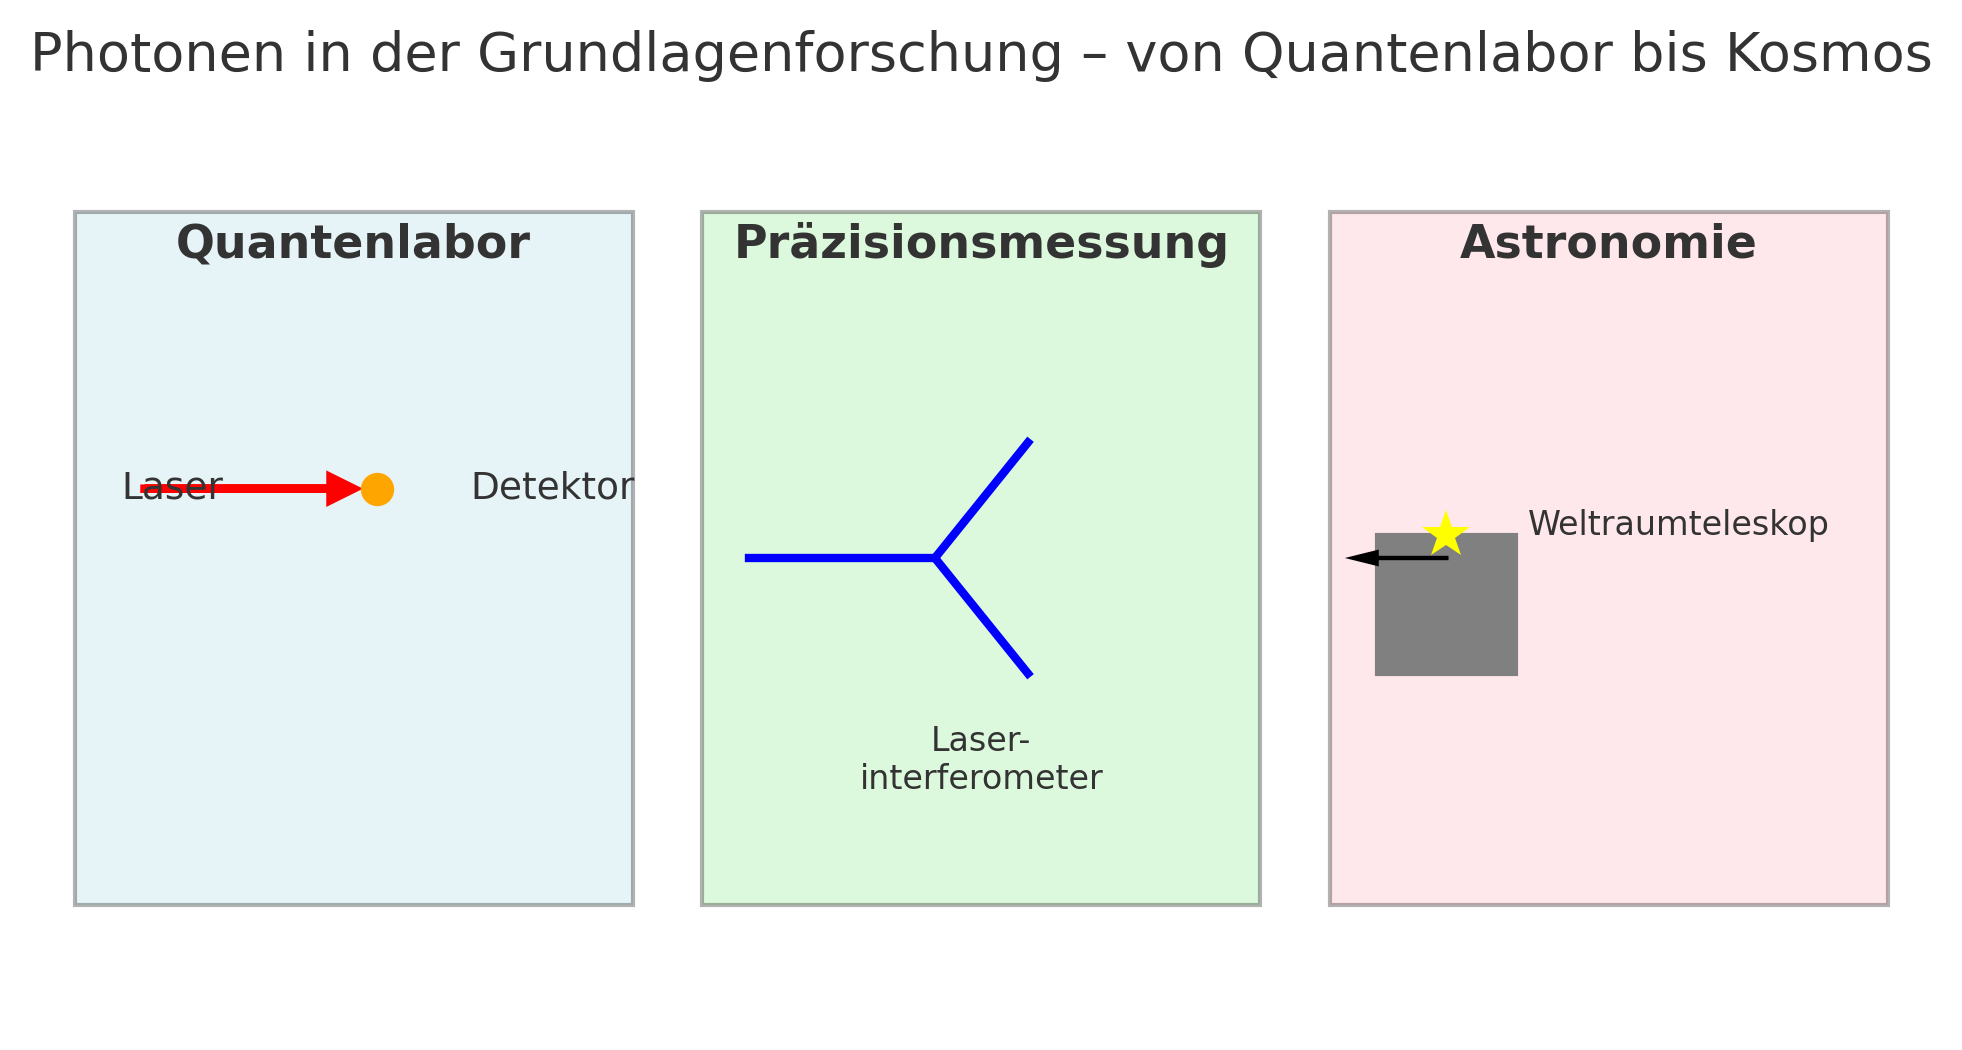
\includegraphics[width=0.9\textwidth]{bilder/photonen_grundlagenforschung.png} % <-- Pfad anpassen
	\caption{Photonen in der Grundlagenforschung: 
		vom Quantenlabor über Präzisionsmessungen bis hin zur Astronomie. 
		Die Illustration zeigt Beispiele für zentrale Einsatzbereiche: 
		Experimente mit einzelnen Photonen im Labor, Laserinterferometrie für Gravitationswellendetektion und weltraumgestützte Beobachtungen von Sternen und Galaxien.}
	\label{fig:photonen_grundlagen}
\end{figure}

\subsubsection{Ausblick}

Die Grundlagenforschung mit Photonen ist längst nicht abgeschlossen. 
Neue Detektionsmethoden, verbesserte Quellen für einzelne und verschränkte Photonen sowie weltraumgestützte Experimente versprechen noch tiefere Einblicke in die Struktur der Naturgesetze.
\newpage
\noindent
\subsection{Ausblick: Graviton, Dunkle Energie, neue \newline Physik?}
\index{Neue Physik}

Auch wenn das Photon als Lichtquant in der modernen Physik bestens verstanden ist, bleiben viele fundamentale Fragen offen – und Photonen spielen bei deren Beantwortung oft eine Schlüsselrolle.

\begin{itemize}
	\item \textbf{Das Graviton:} Das hypothetische Austauschteilchen der Gravitation wurde bisher nicht nachgewiesen. 
	Präzise Messungen mit Photonen – etwa über Gravitationslinsen oder Interferometrie – könnten indirekte Hinweise liefern.
	\item \textbf{Dunkle Energie:} Die beschleunigte Expansion des Universums deutet auf eine bislang unbekannte Form von Energie hin. 
	Photometrie und Spektroskopie entfernter Supernovae und Galaxien nutzen Photonen als einzige Informationsquelle, um diese rätselhafte Komponente zu untersuchen.
	\item \textbf{Neue Physik jenseits des Standardmodells:} Hochpräzise Experimente mit Photonen könnten Abweichungen von etablierten Theorien aufdecken, etwa winzige Verletzungen der Lorentz-Invarianz oder Hinweise auf zusätzliche Raumdimensionen.
\end{itemize}

\begin{tcolorbox}[hypobox, title={Was wäre, wenn das Photon nicht das einzige masselose Boson wäre?}, label={box:photon_neue_physik}]
	\small
	Die Existenz weiterer masseloser Austauschteilchen – etwa des Gravitons – würde unser Verständnis der fundamentalen Kräfte grundlegend verändern. 
	Photonenexperimente könnten über subtile Effekte, wie Abweichungen in der Lichtausbreitung oder Polarisationsmuster, erste Hinweise auf eine solche neue Physik liefern.
\end{tcolorbox}
\begin{figure}[H]
	\centering
	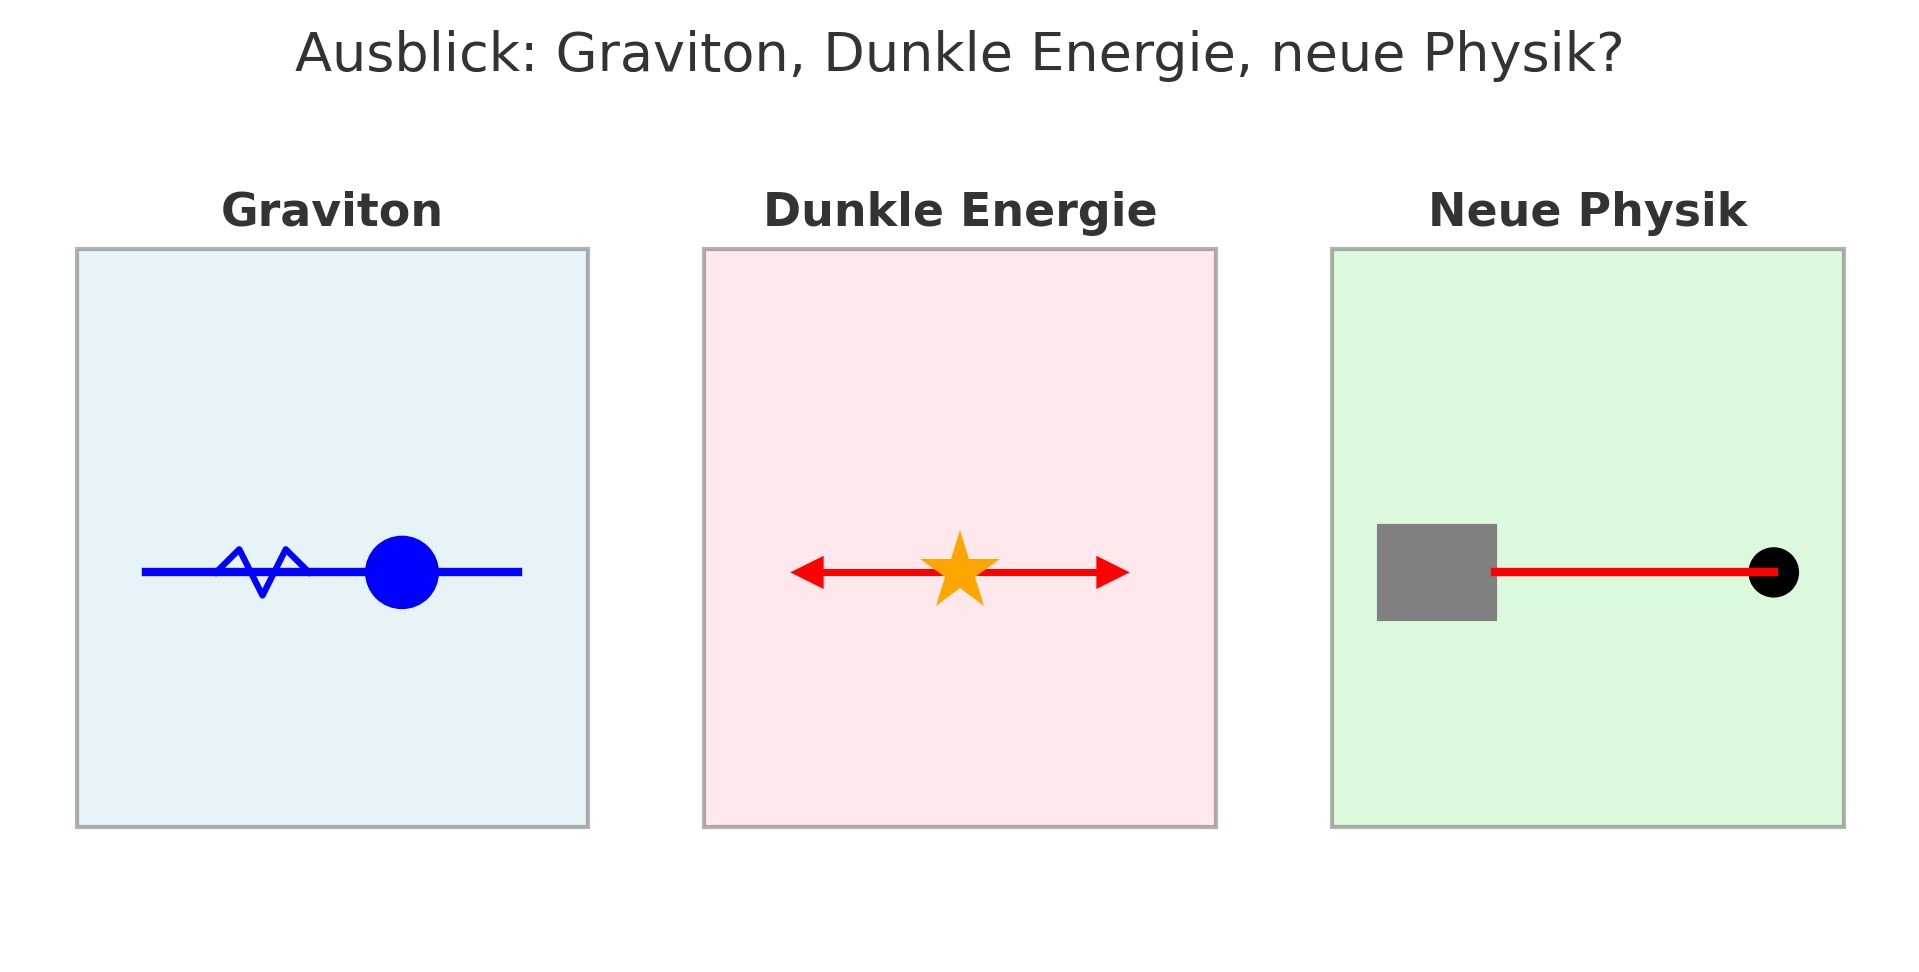
\includegraphics[width=0.9\textwidth]{bilder/photonen_ausblick_fixed.png} % <-- Pfad anpassen
	\caption{Symbolische Darstellung des Ausblicks auf offene Fragen in der Physik:
		\textbf{links:} das hypothetische Graviton als möglicher weiterer masseloser Austauschteilchen-Kandidat;
		\textbf{Mitte:} Dunkle Energie, erkennbar durch die beschleunigte Expansion des Universums;
		\textbf{rechts:} Labor-Experimente mit Photonen, die nach Hinweisen auf neue Physik suchen.}
	\label{fig:photonen_ausblick}
\end{figure}

\subsubsection{Ausblick}

Die Zukunft der Photonenforschung liegt nicht nur in technischen Anwendungen, sondern auch in der Rolle des Photons als präzisem Boten neuer Naturgesetze. 
Weltraumteleskope, Gravitationswellenobservatorien und Labor-Experimente mit nie dagewesener Empfindlichkeit könnten uns der Beantwortung dieser fundamentalen Fragen näherbringen.

\subsection{Fazit}

Photonen sind weit mehr als nur Träger von Licht – sie sind Werkzeuge, Datenüberträger, Messinstrumente und Boten der fundamentalen Gesetze der Natur. 
Von optischer Kommunikation und präziser Messtechnik über photonische Computer bis hin zur Untersuchung kosmischer Phänomene zeigt sich ihre Vielseitigkeit. 
Die hier vorgestellten Anwendungen verdeutlichen, dass Photonen nicht nur die Grundlage moderner Technologien bilden, sondern auch entscheidend für die Erforschung offener Fragen der Physik sind – von der Natur der Gravitation über die Dunkle Energie bis hin zu möglichen Erweiterungen des Standardmodells. 
Die Zukunft der Photonenforschung liegt daher gleichermaßen in der Weiterentwicklung technischer Systeme wie in der Suche nach neuer Physik.

\medskip
\emph{Das Photon ist nicht nur ein Lichtteilchen – es ist ein Schlüssel zur Technologie von heute und zur Physik von morgen.}
\vspace{1em}
\begin{tcolorbox}[hypobox, title={Was wäre, wenn wir Photonen völlig kontrollieren könnten?}]
	\label{box:hypo_kapVII}
	Ein Gedankenexperiment: 
	\begin{itemize}
		\item Photonenchips könnten klassische Elektronik ablösen – mit nahezu lichtschnellen Berechnungen.
		\item Globale Quantenkommunikationsnetze wären absolut abhörsicher.
		\item Einzelphotonen-Labore könnten medizinische Diagnosen auf molekularer Ebene revolutionieren.
		\item Photonen als „Sonden“ könnten uns direkte Einblicke in Dunkle Materie oder die Struktur der Raumzeit geben.
	\end{itemize}
	\medskip
	Solche visionären Szenarien gehen über heutige Technik hinaus – sie bilden die Brücke zum nächsten Kapitel über \emph{Photonen im Standardmodell und visionäre Anwendungen}.
\end{tcolorbox}
